En este capítulo daremos las definiciones necesarias para el desarrollo del proyecto.
Empezamos estableciendo conceptos relacionados con gráficas abstractas y después
hablaremos de gráficas en el plano, explicamos el concepto de tipo de orden y cómo
se utiliza en este trabajo. Finalmente hablaremos del anti-thickness abstracto
y del anti-thickness geométrico.

La estructura más básica que se utiliza en nuestro trabajo son las gráficas abstractas
a las que llamaremos solamente gráficas. La definición se sigue:
\section{Gráfica}
Las siguientes definiciones fueron tomadas de~\cite{Chartrand2008}.

Una \emph{gráfica} $G$ está compuesta por un conjunto $V$ no vacío de objetos a los que llamamos \emph{vértices}
y un conjunto $E$ de parejas de elementos de $V$ a los que llamamos \emph{aristas}. Denotamos
a la arista $e$ compuesta por los vértices $u$ y $v$ como $(u,v)$. Para describir a la gráfica $G$
compuesta por el conjunto $V$ de vértices y el conjunto $E$ de aristas escribimos $G=(V,E)$.
Para referirnos al conjunto de vértices de $G$ escribimos $V(G)$ y para referirnos
al conjunto de aristas de $G$ escribimos $E(G)$. En la figura~\ref{fig:g5vex} podemos observar
un ejemplo de una gráfica con $5$ vértices.

\begin{figure}[t]
  \centering
  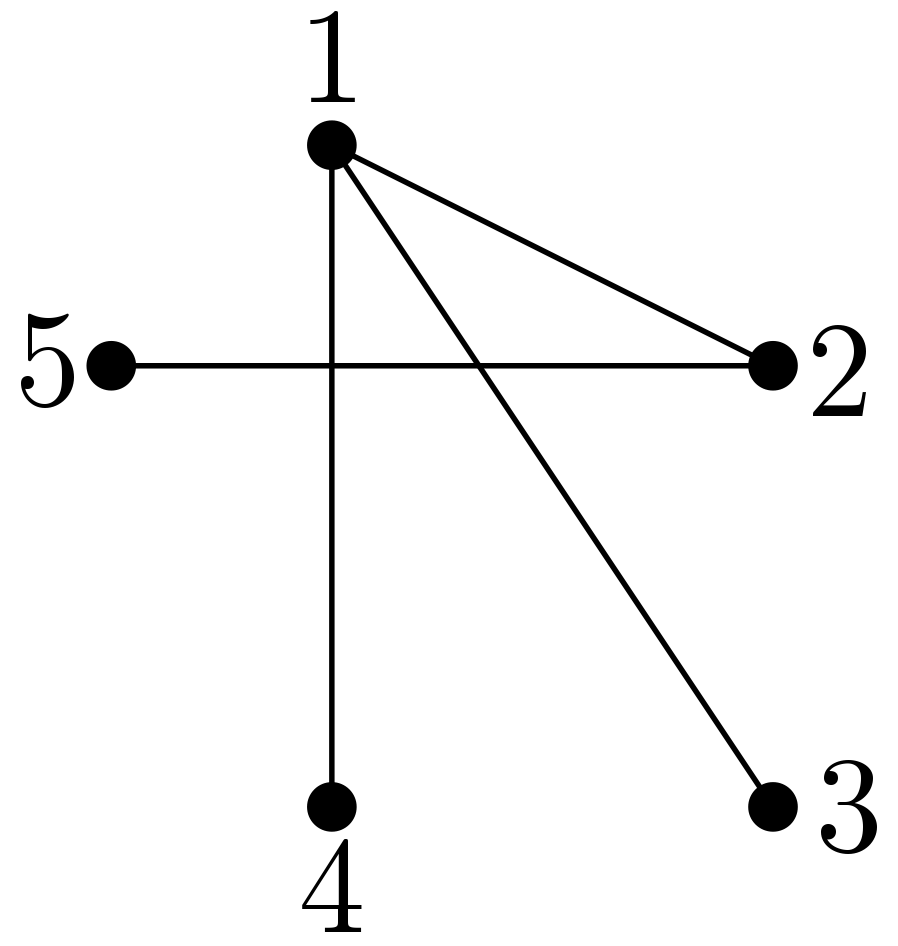
\includegraphics[width=0.3\linewidth]{g5vex.png}
  \caption{Una gráfica de 5 vértices y 4 aristas.}
  \label{fig:g5vex}
\end{figure}

Decimos que dos vértices $u,v\in V(G)$ son \emph{adyacentes} si existe una arista
$(u,v)\in E(G)$. La figura~\ref{fig:exady} muestra un ejemplo de dos vértices adyacentes.
\begin{figure}[htb]
  \centering
  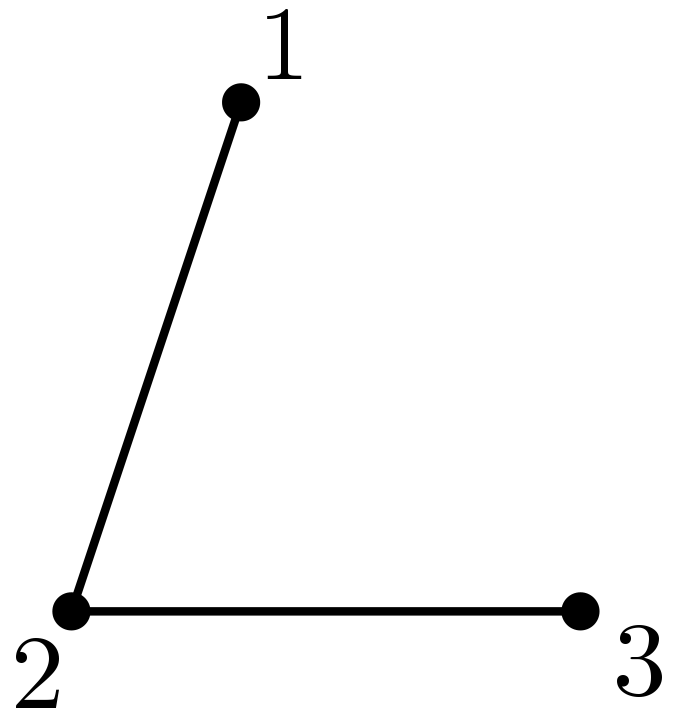
\includegraphics[width=0.3\linewidth]{exady}
  \caption{En esta gráfica el vértice $1$ es adyacente con el vértice $2$ pero
  no es adyacente con el vértice $3$.}
  \label{fig:exady}
\end{figure}
Decimos que dos aristas $e_1,e_2 \in E(G)$ son adyacentes
si inciden en el mismo vértice. Una gráfica es \emph{completa} si cada pareja de vértices
en la gráfica es adyacente. La figura~\ref{fig:exadycomplete} exhibe un ejemplo de adyacencia de
aristas y un ejemplo de una gráfica completa. Para referirnos a la gráfica completa de $n$
vértices escribimos $K_n$. Una gráfica $G$ es \emph{bipartita} si es posible
dar una partición de $V(G)$ en dos subcojuntos $U$ y $W$ de tal manera que cada
arista de $G$ tenga un extremo en $U$ y otro extremo en $W$. Podemos observar
un ejemplo de gráfica bipartita en la figura~\ref{fig:exbipar}.
\begin{figure}[htb]
  \centering
\begin{subfigure}[h]{.4\textwidth}
  \centering
  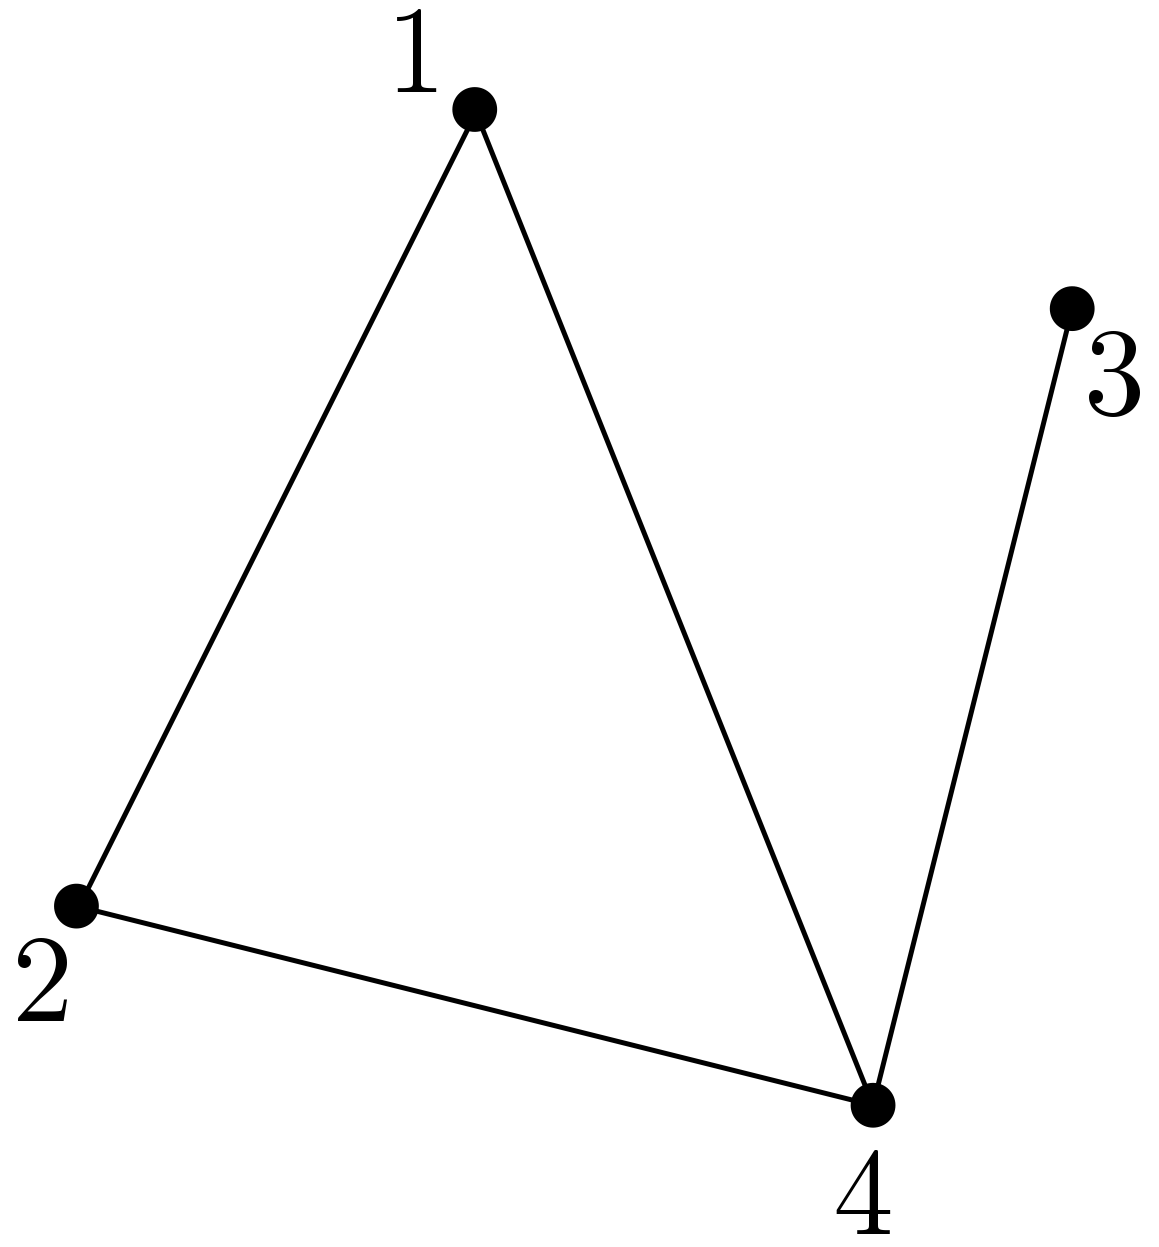
\includegraphics[width=.6\linewidth]{exadyedge}
  \caption{La arista $(1,2)$ es adyacente con las aristas $(2,4)$ y $(1,4)$ pero
  no es adyacente con la arista $(3,4)$.}
  \label{fig:exadyedge}
\end{subfigure}\hfill%
\begin{subfigure}[h]{.4\textwidth}
  \centering
  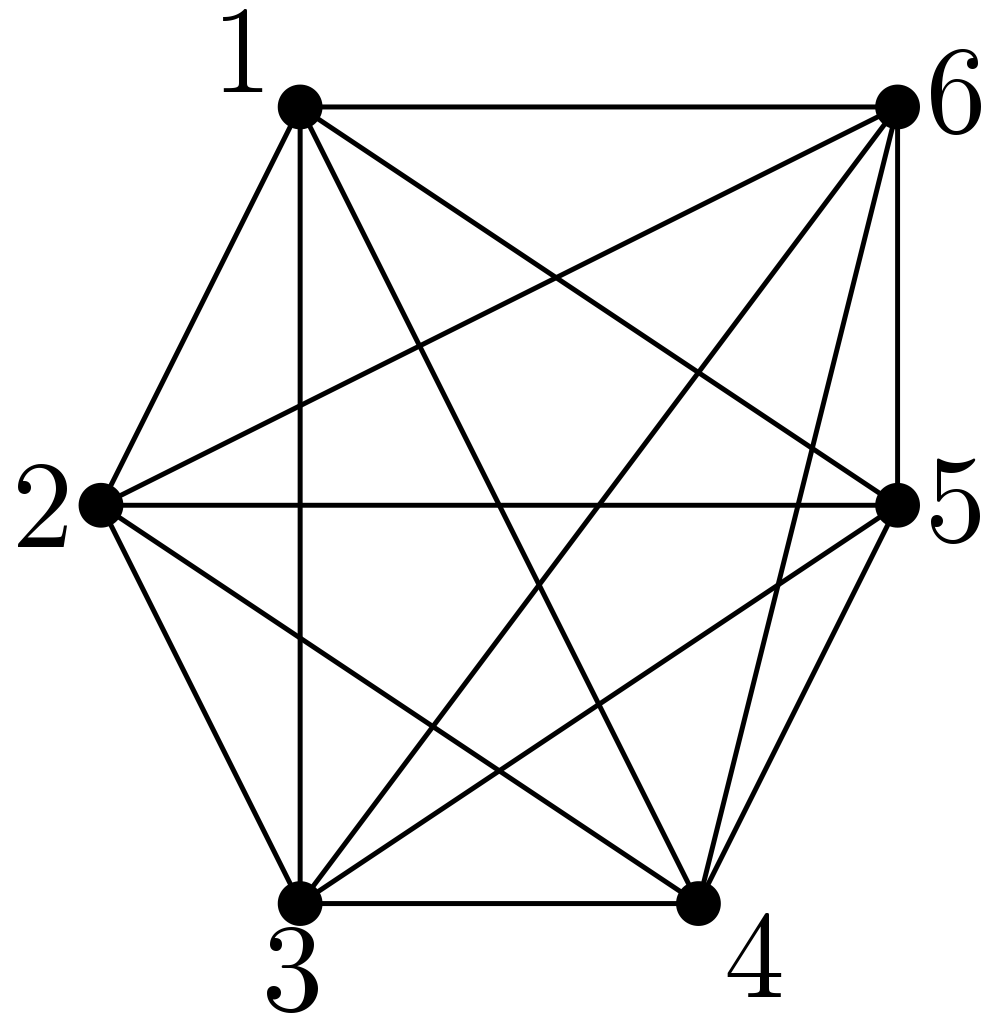
\includegraphics[width=.6\linewidth]{excomplete}
  \caption{La gráfica completa de 6 vértices tiene una arista por cada par de vértices.}
  \label{fig:excomplete}
\end{subfigure}
\caption{Un ejemplo de adyacencia y de una gráfica completa, en la gráfica completa
ocurren todas las adyacencias posibles entre pares de vértices.}
\label{fig:exadycomplete}
\end{figure}
\begin{figure}[h]
  \centering
  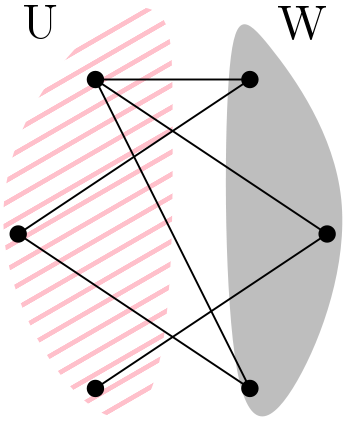
\includegraphics[width=0.3\linewidth]{exbipartita}
  \caption{Un ejemplo de una gráfica bipartita, con conjuntos $U$ y $W$, ambos de tamaño 3.}
  \label{fig:exbipar}
\end{figure}

Una \emph{descomposición} $D$ de una gráfica $G$ es una colección $D=\{G_1,G_2,\dots,G_k\}$ de
subgráficas de $G$ tal que cumple con dos condiciones:
\begin{enumerate}
  \item Ninguna subgráfica $G_i$ contiene vértices aislados.
  \item Cada arista de $G$ pertenece a exactamente una subráfica $G_i$ de $D$.
\end{enumerate}

La figura~\ref{fig:exdecom} ilustra un ejemplo de una descomposición de la gráfica $K_4$.
\begin{figure}[htbp]
  \centering
  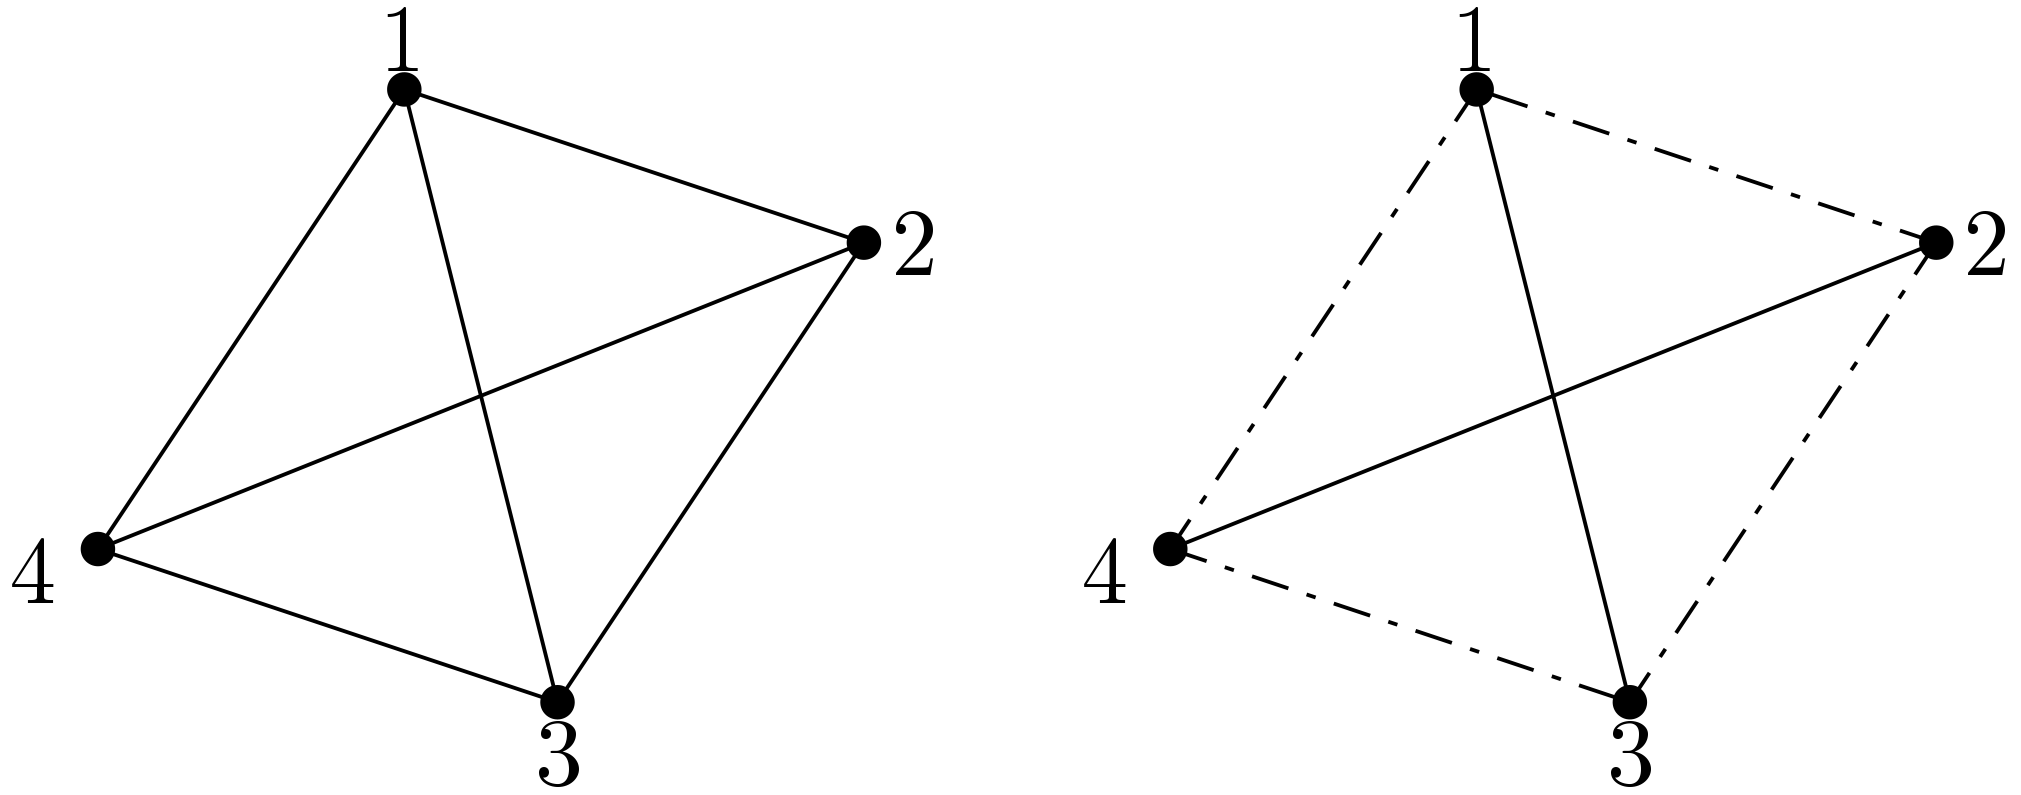
\includegraphics[width=0.7\linewidth]{exdecom}
  \caption{Un ejemplo de una descomposición de $K_4$ en dos gráficas. Una
  compuesta por las aristas $(1,4),(1,2),(2,3),(3,4)$ y otra compuesta por las aristas $(1,3),(2,4)$.}
  \label{fig:exdecom}
\end{figure}
\section{Gráfica geométrica}
Los primeros dos párrafos de esta sección fueron tomados de de~\cite{Pach2013}. El tercer párrafo
fue extraido de~\cite{Lara2019}. El cuarto párrafo fue tomado de~\cite{Pach2011}.
Un \emph{dibujo} $\mathsf{G}=(V,E)$ de una gráfica $G$ es una representación de la
gráfica $G$ en el plano. Cada vértice de $G$ es representado por un punto en el plano
y cada arista de $G$ es representada como una curva simple continua que conecta un par de vértices.
El conjunto de vértices y el conjunto de aristas de $\mathsf{G}$
son los puntos y las curvas respectivamente. Sin perdida de generalidad nos referimos al
conjunto de puntos de $\mathsf{G}$ como $V(\mathsf{G})$ y les llamamos vértices y nos
referimos al conjunto de curvas de $\mathsf{G}$ como $E(\mathsf{G})$ y les llamamos aristas.

Cuando restringimos dichas curvas a segmentos de recta el dibujo de la gráfica
adquiere el nombre de \emph{gráfica geométrica}. Una gráfica
geométrica es completa si existen segmentos de recta entre cada par de vértices
de $V(\mathsf{G})$. En la figura~\ref{fig:exdrawk5} podemos observar un dibujo de $K_5$ y una
gráfica geométrica de $K_5$.
\begin{figure}[htpb]
  \centering
  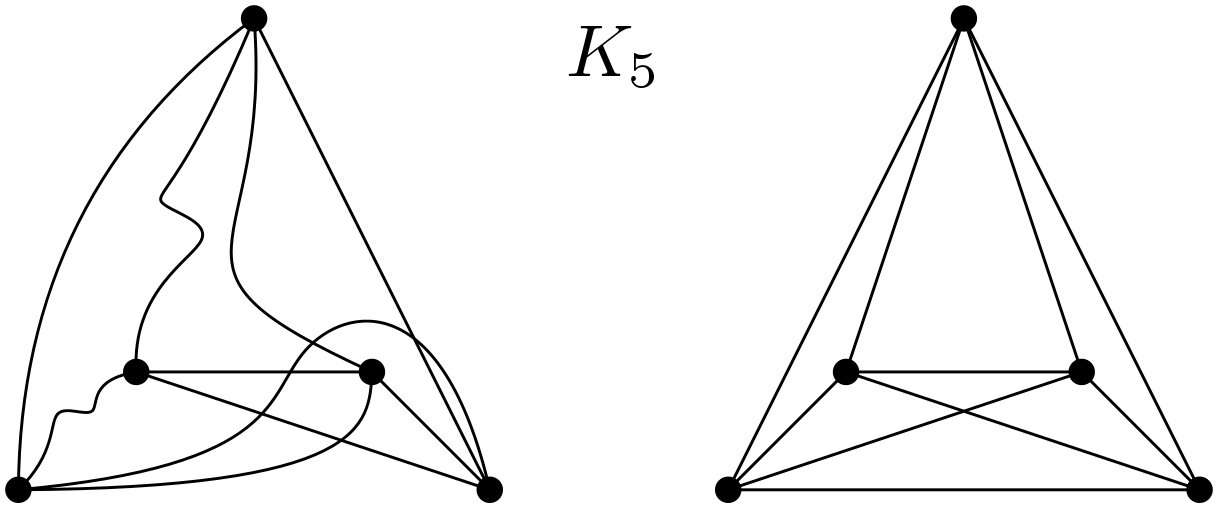
\includegraphics[width=0.8\linewidth]{exdrawk5}
  \caption{En la izquierda observamos un dibujo de $K_5$ y en la derecha observamos
  una gráfica geométrica de $K_5$.}
  \label{fig:exdrawk5}
\end{figure}

Sea $S$ un conjunto de $n$ puntos en el plano en posición general y sea $\mathsf{G}$
una gráfica geométrica. Decimos que $G$ está definida sobre $S$ si $V(\mathsf{G}) = S$.
Podemos notar que cualquier conjunto de puntos $S$ en posición
general induce una gráfica completa.

Decimos que dos aristas $e_1,e_2 \in E(\mathsf{G})$ se \emph{cruzan} si existe un punto $p$
en alguna de las aristas tal que en $p$ la arista $e_1$ pasa de un lado de la arista
$e_2$ hacia el otro lado.

En este trabajo decimos que dos aristas de una gráfica geométrica se \emph{intersectan}
si son adyacentes o si se cruzan. La figura~\ref{fig:exintersection} explica un ejemplo de este concepto.
\begin{figure}[htpb]
  \centering
  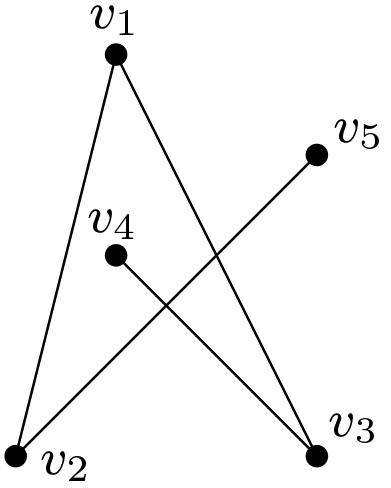
\includegraphics[width=0.3\linewidth]{exintersection}
  \caption{En este ejemplo la arista $(1,2)$ no se intersecta con la arista $(3,4)$
  pero sí se intersecta con la arista $(2,5)$. La arista $(2,5)$ sí intersecta a la arista
  $(3,4)$}
  \label{fig:exintersection}
\end{figure}
% Sin perdida de generalidad
% representamos a una gráfica geométrica como $\mathsf{G}$ y nos referimos a su
% conjunto de vértices como $V(\mathsf{G})$ y a su conjunto de aristas como
% $E(\mathsf{G})$.

\section{Thrackles}
Dado un dibujo $\mathsf{G}$. $\mathsf{G}$ es un \emph{thrackle} si cada par de aristas
se intersecta exactamente una vez. Un thrackle de $n$ vértices
es \emph{máximo} si tiene exactamente $n$ aristas. La figura~\ref{fig:exmaxth} muestra un
thrackle máximo.

\begin{figure}[htpb]
  \centering
  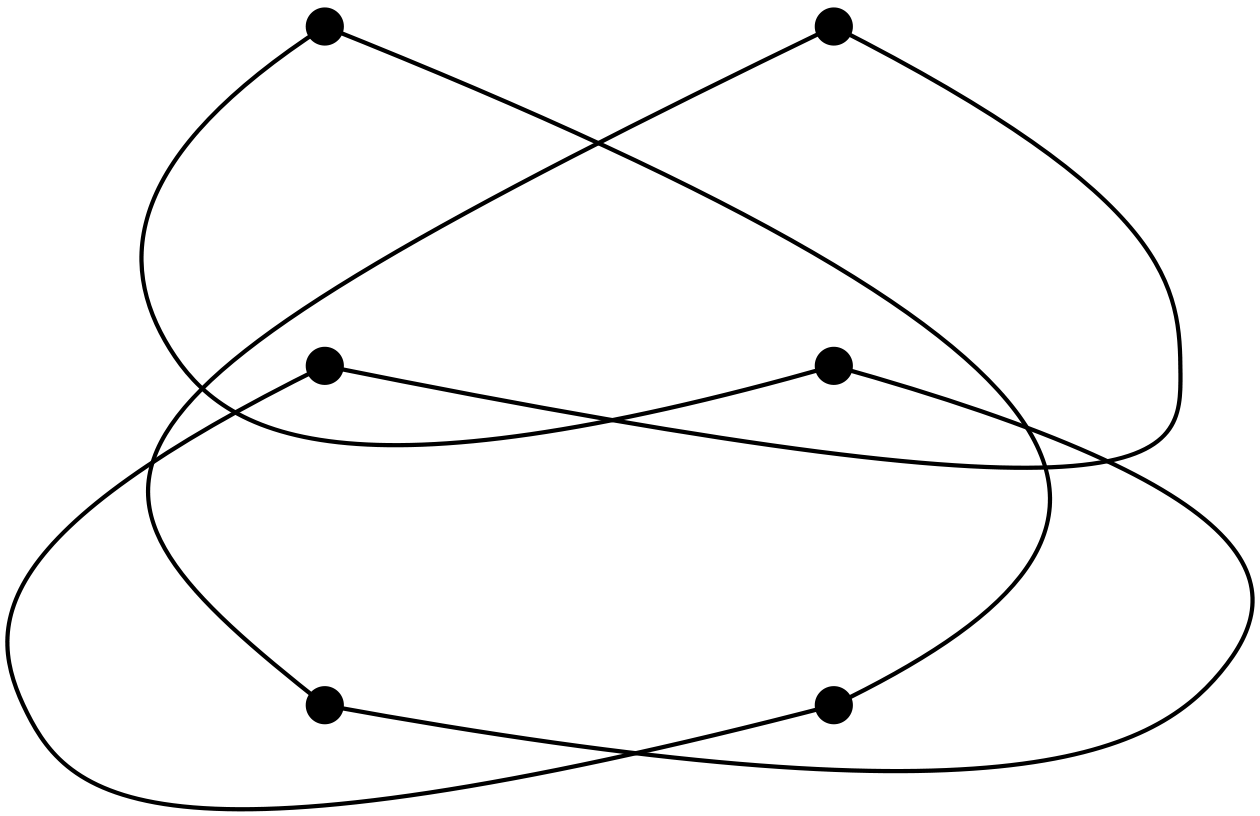
\includegraphics[width=0.35\linewidth]{exmaxth}
  \caption{Un thrackle máximo sobre un conjunto de 5 vértices.}
  \label{fig:exmaxth}
\end{figure}

Un thrackle en el que sus aristas son curvas es conocido como \emph{thrackle topológico}.
Un thrackle en el que todas sus aristas son segmentos de recta es conocido como
\emph{thrackle geométrico}. En este trabajo nos referimos a los thrackles geométricos
como thrackles. En la figura tal podemos notar un ejemplo de thrackle topológico y
un ejemplo de thrackle geométrico.

\begin{figure}[htb]
  \centering
\begin{subfigure}[h]{.4\textwidth}
  \centering
  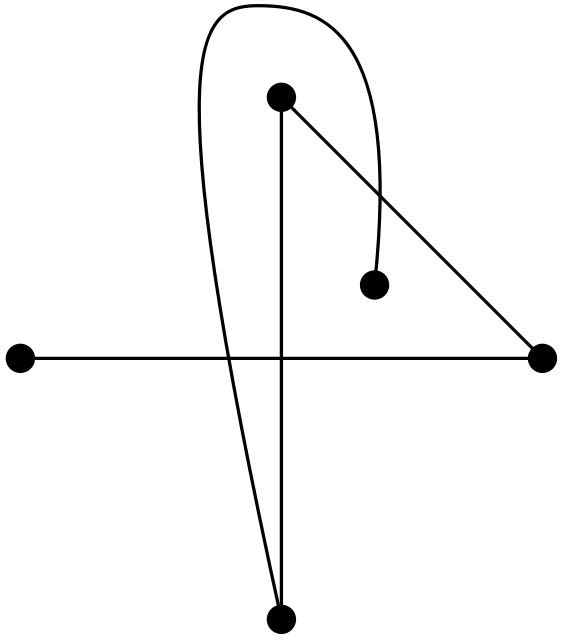
\includegraphics[width=.6\linewidth]{exthtop}
  \caption{Un thrackle topológico sobre conjunto de 5 vértices.}
  \label{fig:exthtop}
\end{subfigure}\hfill%
\begin{subfigure}[h]{.4\textwidth}
  \centering
  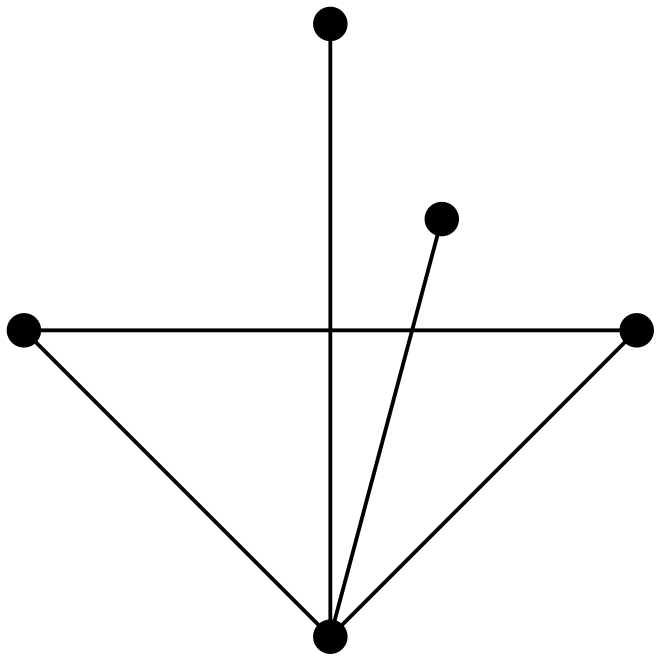
\includegraphics[width=.6\linewidth]{exthgeo}
  \caption{Un thrackle geométrico sobre el mismo conjunto de 5 vértices.}
  \label{fig:exthgeo}
\end{subfigure}
\caption{Ambas figuras ilustran thracklese definidos sobre el mismo conjunto de
puntos. En los dos casos el thrackle dibujado es máximo.}
\label{fig:exthgeotop}
\end{figure}

Una descomposición por thrackles $D$ de una gráfica geométrica
$\mathsf{G}$ es una colección $D=\{\mathsf{G}_1,\mathsf{G}_2,\dots,\mathsf{G}_k\}$
de subgráficas que cumple con tres condiciones:
\begin{enumerate}
  \item Cada subgráfica $\mathsf{G}_i$ es un thrackle.
  \item Ninguna subgráfica $\mathsf{G}_i$ contiene vértices aislados.
  \item Cada arista de $\mathsf{G}$ pertenece a exactamente una subráfica $\mathsf{G}_i$ de $D$.
\end{enumerate}

Una gráfica $G$ es \emph{thrackleable} si puede ser dibujada en el plano como un thrackle.
\section{Tipo de Orden}
\section{Anti-thickness y anti-thickness geométrico}
Las siguientes definiciones fueron tomadas de~\cite{Dujmovic2017}.

El \emph{anti-thickness} de una gráfica $G$ es el entero $k$ más pequeño tal que existe una
partición de $E(G)$ de tamaño $k$ en la que cada elemento de la partición
es una gráfica thrackleable. La figura~\ref{fig:exantithickness} ilustra un ejemplo del
anti-thickness de $K_5$.
\begin{figure}
  \centering
  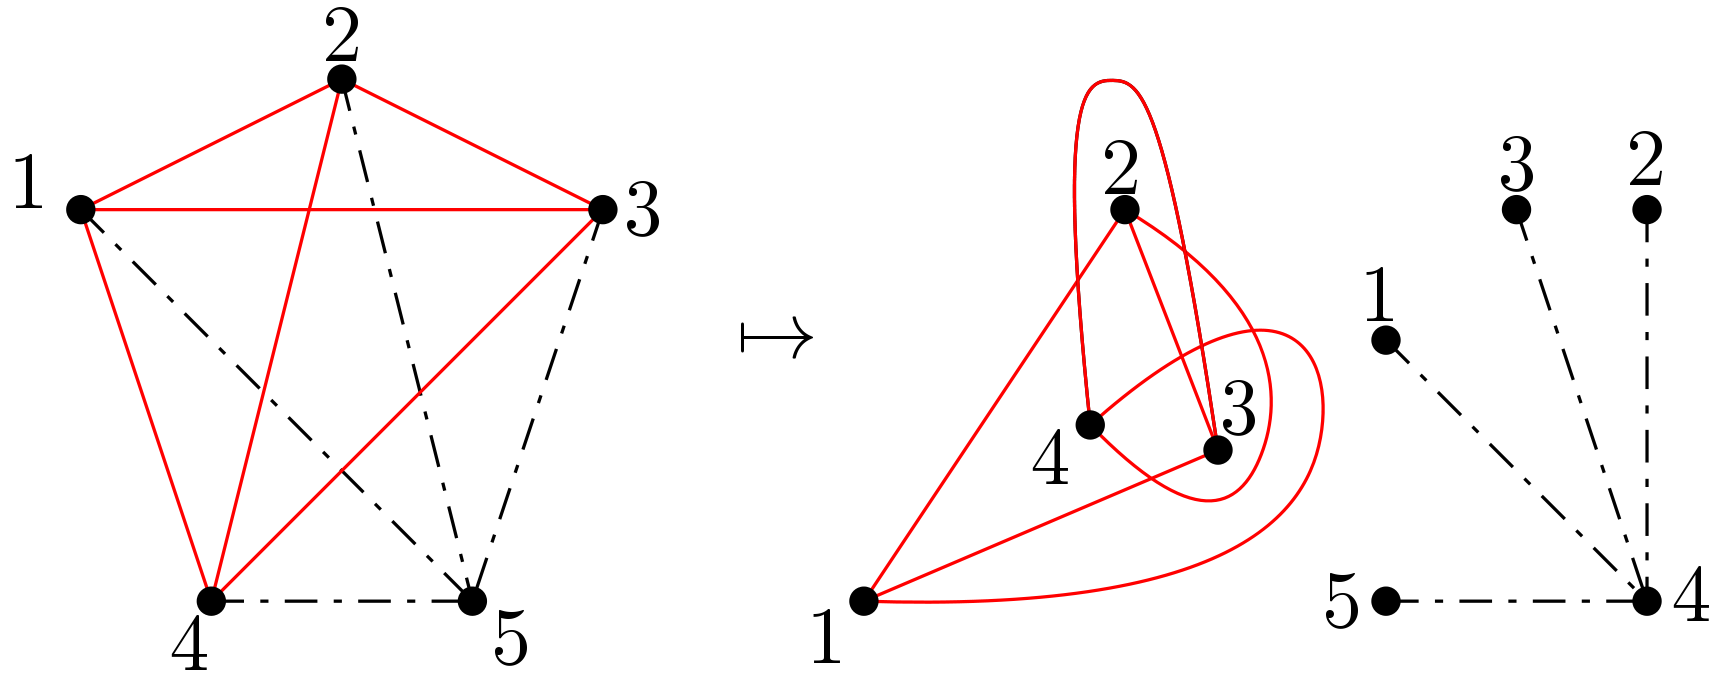
\includegraphics[width=0.9\linewidth]{exantithickness}
  \caption{Las aristas de la gráfica completa inducida por los vértices $1,2,3,4$
  inducen un thrackle topológico (dibujado con lineas continuas)
  mientras que las aristas con un extremo en el vértice $5$ inducen un thrackle geométrico
  (dibujado con lineas punteadas).
  El anti-thickness de $K_5$ es precisamente igual a dos.}
  \label{fig:exantithickness}
\end{figure}

El \emph{anti-thickness} geométrico de una gráfica $G$ es el entero $k$ más pequeño tal que existe un
dibujo $\mathsf{G}$ de $G$ para el cual hay una partición de $E(\mathsf{G})$ de tamaño $k$
en la que cada elemento de la partición es un thrackle.
\section{Número cromático}
